\tikzset{every picture/.style={line width=0.75pt}} %set default line width to 0.75pt        
\begin{center}
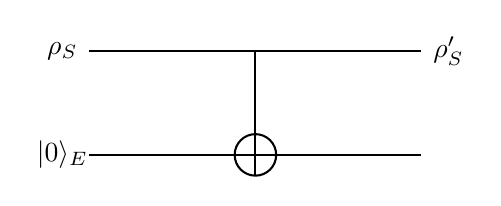
\begin{tikzpicture}[x=0.75pt,y=0.75pt,yscale=-1,xscale=1]
%uncomment if require: \path (0,300); %set diagram left start at 0, and has height of 300

%Straight Lines [id:da5839193375924283] 
\draw    (230,120) -- (390,120) ;


%Straight Lines [id:da5250417297428058] 
\draw    (230,170) -- (390,170) ;


%Straight Lines [id:da6806435798614072] 
\draw    (310,120) -- (310,170) ;


%Flowchart: Or [id:dp38998241497199526] 
\draw   (300,170) .. controls (300,164.48) and (304.48,160) .. (310,160) .. controls (315.52,160) and (320,164.48) .. (320,170) .. controls (320,175.52) and (315.52,180) .. (310,180) .. controls (304.48,180) and (300,175.52) .. (300,170) -- cycle ; \draw   (300,170) -- (320,170) ; \draw   (310,160) -- (310,180) ;

% Text Node
\draw (217,120) node   {$\rho_S$};
% Text Node
\draw (217,170) node   {$|0\rangle_E$};
% Text Node
\draw (403,120) node   {$\rho'_S$};


\end{tikzpicture}
\end{center}